\chapter[Proposta]{Proposta}
Este capítulo apresenta detalhes sobre o \textit{framework} proposto neste trabalho de conclusão de curso. O capítulo está organizado em seções. Na seção 4.1, é explanado sobre a visão geral do \textit{framework}. Em seguida, nas seções 4.2 e 4.3, são apresentados a linguagem alvo inicial \textit{Grails} e a notação candidata para especificar os casos de teste usando o \textit{framework}, respectivamente. Na seção 4.4, é explanado sobre a prova de conceito realizada com o intuito de verificar a viabilidade do projeto. Por fim, na seção 4.5,  são apresentados os resultados obtidos até o momento.

\section{Framework para Geração de Teste Unitário} \label{ch4sec1}

A proposta deste trabalho é a implementação de um \textit{framework} capaz de dar suporte ao desenvolvedor na tarefa de produzir testes unitários.  Esse suporte possibilitará a geração de testes de forma semiautomatizada, visto que o programador deverá incluir no código especificações que guiem o \textit{framework} na criação dos testes unitários. 
\par
\indent A princípio, o \textit{framework} será desenvolvido com o intuito de gerar testes unitários em aplicações escritas em \textit{Grails}, especificamente para as operações básicas conhecidas como CRUD (\textit{create}, \textit{read}, \textit{update} e \textit{detele}). Entretanto, há intenção de evoluir o \textit{framework} para que ele seja compatível com demais métodos e linguagens de programação. 
\par
\indent Para a implementação do \textit{framework}, será utilizada a linguagem de programação C++, junto com as ferramentas Flexc++ \cite{flexcpp2015} e Bisonc++ \cite{bisoncpp2015}. A Figura 4 fornece uma visão geral das camadas do \textit{framework}.
 
 \begin{figure}[h]
    \centering
    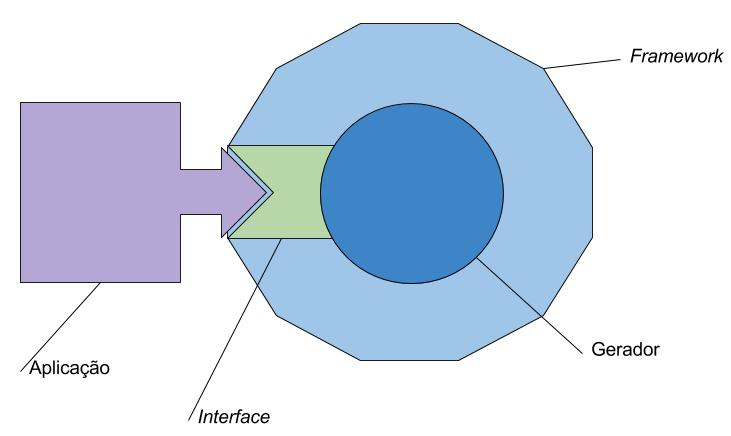
\includegraphics[width=0.7\textwidth]{figuras/estruturaarquitetural.jpg}
    \caption{Camadas do \textit{Framework}}
    \label{fig:estruturaarquitetural}
 \end{figure}

 \par
 \indent O \textit{framework} proposto será constituído essencialmente por duas camadas: uma camada para \textbf{geração de testes} e uma camada para \textbf{customização}. A camada de geração de testes é o núcleo do \textit{framework}. Essa camada é responsável por produzir os testes especificados, enquanto que a camada mais de customização, mais 
 
   \begin{figure}[h]
    \centering
    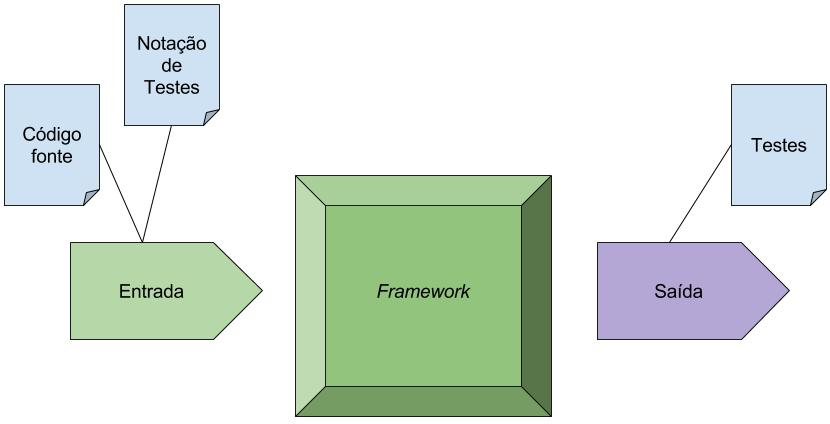
\includegraphics[width=0.7\textwidth]{figuras/entradasesaidas.jpg}
    \caption{Fluxo do funcionamento do \textit{Framework}}
    \label{fig:entradasesaidas}
 \end{figure}
 
 \par
\indent A Figura \ref{fig:entradasesaidas} enfatiza o fluxo do funcionamento do \textit{framework}. A entrada do \textit{framework} será o código fonte, bem como as especificações dos testes seguindo uma notação pré-determinada. Como saída, serão gerados os testes unitários conforme especifícados. O fluxo do funcionamento do \textit{framework} pode ser entendido, de forma simplificada, em quatro módulos: análise léxica, análise sintática, análise semântica e geração dos testes. 
 \begin{description}
 \item[Análise léxica:] onde será realizada a análise do código fonte de forma a reconhecer as palavras específicas, os \textit{tokens}. Essas palavras serão previamente definidas por meio do Flexc++ que fornece suporte para essa etapa \cite{flexcpp2015}.
 \item[Análise sintática:] ocorrerá uma avaliação do código fonte considerando as regras sintáticas definidas. Essas regras são formadas utilizando sequências de \textit{tokens}. Essa etapa será implementada com o auxílio do Bisonc++ \cite{bisoncpp2015}.
 \item[Análise semântica:] será realizada uma interpretação do código apresentado verificando sua semântica, ou seja, será averiguado o significado dos \textit{tokens} identificados dentro do contexto.
  \item[Geração dos testes:] após as análises do código, será efetuado o \textit{parser} com o intuito de gerar os testes unitários especificados pelo desenvolvedor. Esses testes serão armazenados nos arquivos apropriados e representarão a principal saída do \textit{framework}.
 \end{description}
 
 \begin{figure}[h]
    \centering
    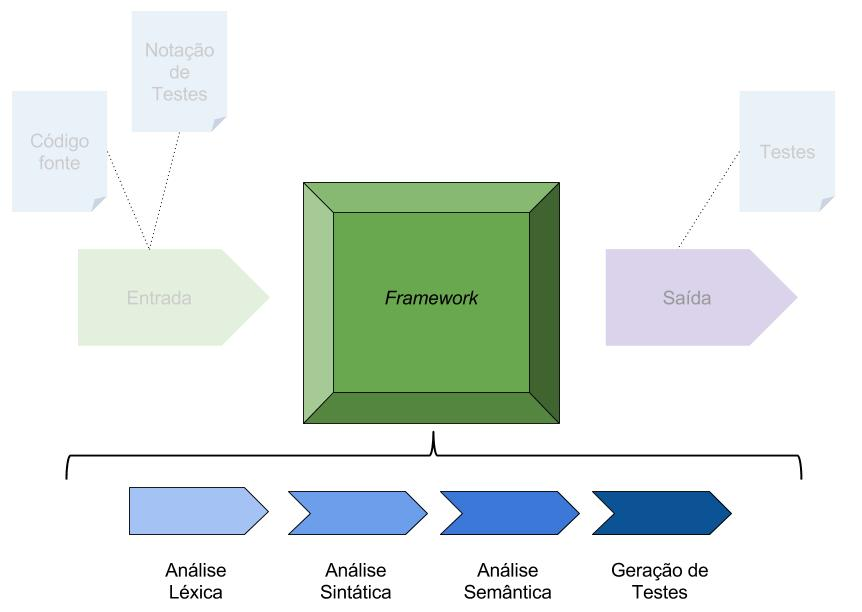
\includegraphics[width=0.9\textwidth]{figuras/Framework-interior (1).jpg}
    \caption{Fluxo do Funcionamento do \textit{Framework}}
    \label{fig:Framework-interior}
 \end{figure}
 
 \par
 \indent A Figura \ref{fig:Framework-interior} permite a visualização do fluxo básico do funcionamento do \textit{framework}.  

\section{Alvo Inicial: \textit{Grails}} 
\textit{Grails}, antigamente conhecido como \textit{Groovy on Grails}, é um \textit{web framework} para plataforma Java. Com o objetivo de propiciar maior produtividade ao desenvolvedor, \textit{Grail} faz uso do paradigma \textit{Convention-over-Configuration}.  Por ser integrado com a JVM (\textit{Java Virtual Machine}), \textit{Grails} possui diversas características, entre elas: a integração com ORM (\textit{Object Relational Mapping}), uso de uma \textit{domain-specific-language} e programação assíncrona \cite{grails2015}.
\par
\indent Devido ao fato de ser um \textit{web framework}, \textit{Grails} faz uso do padrão MVC (\textit{Model-View-Controller}), ou seja, as aplicações em \textit{Grails} separam a interação com usuário da representação da informação \cite{grails2015}.
\par
\indent \textit{Grails} utiliza-se de um sistema de comandos capaz de fornecer ao desenvolvedor a possibilidade de gerar código. Isso evita tarefas monótonas, mas necessárias, como funções básicas de \textit{models} e de \textit{controllers}. Esses métodos gerados podem ser modificados pelo desenvolvedor, conforme a necessidade de adequação ao contexto de trabalho  \cite{grails2015}.
\par
\indent Os geradores de código do \textit{Grails} produzem  \textit{stubs} para os testes. \textit{Stubs} são métodos ou classes vazias, contendo apenas cabeçalhos. Ao analisar os \textit{stubs} gerados, observa-se que eles são classes filhas do \textit{GroovyTestCase} que, por sua vez, é um \textit{facade} sobre o JUnit \cite{broughton2010}. Devido a isso, qualquer desenvolvedor que esteja familiarizado com o uso de funcionalidades comuns ao JUnit, como \textit{asserts}, \textit{setup} e \textit{teardown}, está apto a entender os testes em \textit{Grails} \cite{broughton2010}.
\par
\indent A seguir - Código 4.1 - é apresentado um exemplo de um teste escrito utilizando o \textit{web framework Grails}:

\begin{lstlisting}[language=java, label=exTesteGrails, caption={Exemplo de Teste em \textit{Grails}}]
// Model
class Restaurant{
  String name
}

// Test
class RestaurantTests extends GroovyTestCase {
  void testSomething(){
    Restaurant restaurant = new Restaurant(name:"Gepetohut")
    assertEquals "Gepetohut", restaurant.name
  }
}
\end{lstlisting}

\section{Especificação dos Casos de Testes}
Como referenciado na seção \ref{ch4sec1}, será utilizada uma notação no código fonte que possibilitará ao desenvolvedor especificar seus casos de teste. Essa notação será inserida em comentários de documentação, permitindo assim, a especificação dos testes e a documentação dos mesmos, tudo centrado no código fonte.
\par
\indent Em essência, o desenvolvedor deverá ser responsável por definir quais serão as entradas dos testes e a saída esperada. Fazendo isso, o \textit{framework} será capaz de identificar esses valores e gerar os testes solicitados.
\par
\indent A seguir - Código 4.2 - consta um exemplo de uma notação candidata, que poderá ser usada para definir os dados de entrada para o \textit{framework}.

\begin{lstlisting}[language=java, label=notacaoCandidata, caption={Notação Candidata}]
/**
 * This method sum two numbers.
 * 
 * @param fisrtParcel a parcel of sum.
 * @param secondParcel a parcel of sum.
 * @return result the result of sum.
 * 
 * scarefault.test
 *   scenario: "sum two valid numbers"
 *     scarefault.entries: 2, 2
 *     scarefault.out: 4
 *
 *   scenario: "sum zeros"
 *     scarefault.entries: 0, 0
 *     scarefault.out: 0
 */
def addTwoNumbers(Integer firstParcel, Integer secondParcel) {
   result = firstParcel + secondParcel
   return result
}

// Test
void sumTwoValidNumbers() {
  expectedResult = 4
  result = addTwoNumbers( 2, 2 )
  
  assertEquals expectedResult, result
}

void sumZerosTest() {
  expectedResult = 0
  result = addTwoNumbers( 0, 0 )
  
  assertEquals expectedResult, result
}
\end{lstlisting}

\section{Prova de Conceito}

Para averiguar a viabilidade da implementação do \textit{framework} proposto, foi planejada a execução de uma prova de conceito. Com o objetivo de verificar se as ferramentas, Bisonc++ e Flexc++, atenderão à expectativa no desenvolvimento do \textit{framework}, tornou-se necessário realizar provas de conceito com elas também. 

\subsection{Flexc++} \label{flexcpp}
O Flexc++ é um analisador léxico que é diferente do Flex, pois gera código em linguagem de programação C++. A prova de conceito dessa ferramenta foi produzida em etapas: um estudo sobre o Flexc++, seguido de sua instalação e configuração e, por fim, a execução de um exemplo recomendado pelo \textit{site} oficial.
\par
\indent Com o estudo, constatou-se que o Flexc++ se assemelha ao Flex. Com isso, o seu uso é viável no projeto, já que se possui conhecimento prévio da ferramenta. No Apêndice A constam os resultados desse estudo.
\par
\indent Após a sua instalação, foi implementado um identificador de \textit{tokens} utiizando apenas o Flexc++. Para isso, definiu-se o analisador léxico apresentado a seguir em Código 4.3.:

\begin{lstlisting}[language=C++, label=analisadorPCF, caption={Analisador Léxico da Prova de Conceito do Flexc++}]
%%
[_a-zA-Z][_a-zA-Z0-9]* return 1;
\end{lstlisting}
\par
\indent O Código \ref{analisadorPCF} faz uso de uma expressão regular, \textit{regex}, que identifica qualquer termo alfanumérico. Caso encontre, ele retorna o dígito um, provocando  a chamada da função \textit{match}.
\par
\indent Com a compilação do Flexc++ gera-se uma classe: \textit{Scanner}. Para a demonstração do uso dessa classe, foi implementado um arquivo em linguagem de programação C++ contendo uma função \textit{main} que a utiliza. A seguir - em Código 4.4 - é apresentado o código citado.
\begin{lstlisting}[language=C++, label=mainPCF, caption={Função \textit{main} para demonstração do Flexc++}]
#include <iostream>
#include "Scanner.h"

using namespace std;

int main()
{
  Scanner scanner;
  while( scanner.lex() )
  {
    cout << "[Identifier: " << scanner.matched() << "]";
  }
}
\end{lstlisting}
\par
\indent O código implementado teve o comportamento conforme o esperado.

\subsection{Bisonc++}
Como referenciado na seção \ref{suporteGeracao}, o Bisonc++ é um gerador de \textit{parsers} capaz de converter uma gramática de contexto livre em uma classe \textit{parser} em linguagem C++. A prova de conceito dessa ferramenta é composta pela realização de um estudo, da instalação e configuração da ferramenta e, enfim, de seu uso em um exemplo simples, sugerido no \textit{site} oficial.
\par
\indent Por meio do estudo, foi averiguado que a estrutura do arquivo de entrada do Bisonc++ é semelhante à estrutura do Bison. Dessa forma, constatou-se que a curva de aprendizagem seria aceitável, na medida em que já se tem conhecimento prévio do uso do Bison. Todo o levantamento efetuado por esse estudo consta no Apêndice A.
\par
\indent A instalação do Bisonc++ foi realizada em uma máquina virtual que, por sua vez, foi estabelecida com o auxílio do Vagrant. Com a execução dessa etapa, foi iniciada a configuração de um \textit{script} para automatizar a instalação. O tipo de \textit{script} utilizado foi Makefile, comum na automação de tarefas de construção e compilação de programs em C/C++. Para o funcionamento adequado do Bisonc++ foi necessária a integração dele com o Flexc++, descrito na subseção \ref{flexcpp}.
\par
\indent O uso do Bisonc++ foi realizado por meio da implementação de um identificador de \textit{tokens}. Inicialmente, foi produzido o analisador léxico utilizando o Flexc++. Em Código 4.5 é apresentado o código resultante.

\begin{lstlisting}[language=C++, label=analisadorLexicoPCB, caption=Analisador Léxico da Prova de Conceito do Bisonc++]
%%

[ \t\n]+                            // skip white space chars.
[0-9]+                              return Parser::NUMBER;
[[:alpha:]_][[:alpha:][:digit:]_]*  return Parser::IDENTIFIER;
.                                   return Parser::CHAR;
\end{lstlisting}

\par 
\indent O analisador sintático é onde estão definidas as regras gramáticais. Ele possibilita identificar se a sequência de \textit{tokens} corresponde a uma regra específica e, a partir disso, é realizada uma ação. As regras da prova de conceito do bisonc++ foram definidas da seguinte forma:
\begin{description}
\item[startrule:] permite a leitura completa do arquivo de entrada. Para isso, faz-se uso de recursividade. Essa é a regra inicial, onde é definido que o arquivo de entrada deve ser uma regra \textit{tokenshow} ou ela mesma seguida de uma regra \textit{tokenshow}.
\item[tokenshow:] é definido como um \textit{token} que, ao ser identificado, provoca a ação de impressão do mesmo.
\item[token:] é caracterizado como sendo um identificador, um número ou um caractere. Esses elementos são definidos no Flexc++.
\end{description} 

\begin{lstlisting}[language=C++, label=analisadorSintaticoPC, caption=Analisador Sintático da Prova de Conceito do Bisonc++]
%scanner                ../scanner/Scanner.h
%scanner-token-function d_scanner.lex()

%token IDENTIFIER
%token NUMBER
%token CHAR

%%

startrule:
  startrule tokenshow
|
  tokenshow
;

tokenshow:
  token
  {
    std::cout << "Matched: " << d_scanner.matched() << "\n";
  }
;

token:
  IDENTIFIER
|
  NUMBER
|
  CHAR
;
\end{lstlisting}
\par
\indent O código listado em \ref{analisadorSintaticoPC} é o resultado da implementação das regras explicadas anteriormente. Após a compilação desses dois arquivos, foram geradas duas classes em linguagem C++: \textit{Scanner} e \textit{Parser}. Permite-se, com a geração dessas classes, a customização desses arquivos conforme necessidade.
\par
\indent Para a demonstração do uso das classes geradas foi implementada uma função \textit{main} que instancia e utiliza tais classes, conforme ilustra o Código 4.7.
\begin{lstlisting}[language=C++, label=mainPCB, caption=Função \textit{main} para demosntração do Bisonc++]
#include "parser/Parser.h"

int main(int argc, char **argv)
{
    Parser parser;
    parser.parse();
}
\end{lstlisting}
\par
\indent O código implementado teve o comportamento conforme o esperado.

\subsection{Gerador de Teste Unitário}
Com o intuito de provar a viabilidade do desenvolvimento do gerador de teste unitário, foi idealizada a implementação de um gerador simples. Ele deve ser capaz de criar testes, conforme especificação, referentes a um método de adição de dois números inteiros, escrito em \textit{Grails}. O código resultando é parte integrante da primeira versão do \textit{framework} proposto. 
\par 
\indent Inicialmente, definiu-se o analisador léxico capaz de identificar as informações necessárias para a geração do teste. A princípio, foram levantadas as palavras-chave e símbolos referenciados na Tabela 1.

\begin{table}[h]
  \tiny
  \centering
  \caption{Palavras-chave e símbolos do analisador léxico inicial}
  \label{keywords}
  \begin{tabular}{| c | c |}
    \hline
    Tipo & Símbolos Identificados\\ \hline
     Símbolos & "(";  ")";  "{";  "}";  "[";  "]";  "," e "." \\
     Palavras-chave &   \textit{package}; \textit{import}; \textit{def}; \textit{Integer}; \textit{return}; \textit{scarefault}, \textit{test}; \textit{scenario}; \textit{entries} e \textit{out} \\ \hline
  \end{tabular}
\end{table}



Em seguida, foram estabelecidas as regras gramáticais para criação do arquivo de teste contendo os casos de testes conforme especificados no arquivo de entrada.
\par 
\indent O gerador produzido na prova de conceito possui apenas os analisadores léxico e sintático. O analisador semântico não faz parte do escopo da prova de conceito.

\section{Resultados Obtidos}
\subsection{Resultados Obtidos com as Provas de Conceito do Flexc++ e Bisonc++}
As provas de conceito realizadas com o intuito de verificar o funcionamento das ferramentas Flexc++ e Bisonc++ foram consideradas bem sucedidas. Ambas possuiam como objetivo identificar \textit{tokens} do arquivo de entrada e imprimi-los, entretanto, o software gerado apenas com o uso do Flexc++ não faz uso de regras sintáticas. 

 \begin{figure}[h]
    \centering
    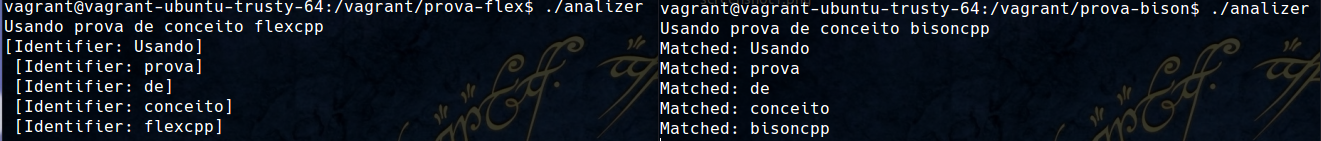
\includegraphics[width=\textwidth,height=3cm]{figuras/resultadosPCBF.png}
    \caption{Resultados das Provas de Conceito sobre Flexc++ e Bisonc++}
    \label{fig:resultadosPCBF}
 \end{figure}

\par
\indent A Figura \ref{fig:resultadosPCBF} apresenta as saídas dos identificadores de \textit{tokens} usando apenas o Flexc++ e o Flexc++ junto com o Bisonc++, respectivamente. É possível observar que ambas foram capazes de identificar as palavras do arquivo de entrada conforme previsto. Obteve-se como principais resultados dessas duas provas de conceito os conhecimentos adquiridos sobre as ferramentas e a integração entre elas, bem como a viabilidade da utilização das mesmas para implementação do \textit{framework} para geração de teste unitário.

\subsection{Resultado Obtido com a Provc de Conceito do Gerador de Teste}

\section{Resumo do Capítulo}
O capítulo abordou sobre a proposta deste trabalho. Com isso, foi explanado sobre como o \textit{framework} funcionará, bem como qual a entrada e saída esperada com o seu uso. Detalhou-se também sobre a linguagem de programação escolhida para geração dos testes unitários e um exemplo de notação candidata que possibilitará o uso do \textit{framework}. Por fim, abordou-se sobre as provas de conceitos desenvolvidas durante o trabalho de conclusão de curso 1 que possuem como objetivo principal constatar a viabilidade do projeto. 

 